\documentclass[aps,tightenlines,16pt]{ctexart}

\usepackage{slashed}
\usepackage{amsmath,amsfonts,amssymb}
% \usepackage{bm}  %黑体希腊字母
\usepackage{bbm} %空心字母数字
\usepackage{ctex}
\usepackage{float}
%\usepackage[dvips]{graphicx}
\usepackage[english]{babel}
\allowdisplaybreaks[4]  %公式环境换行
\numberwithin{equation}{section}
\usepackage{slashed} %费曼slashed
\usepackage[left=2cm,right=2cm,top=2.54cm,bottom=2.54cm]{geometry}
%\usepackage[dvipdfm,pdfstartview=FitH]{hyperref}
%\usepackage{cancel}
%\usepackage{forest}
%\usepackage{leftidx}  %设置上下标
\usepackage{cite}
\usepackage[justification=centering]{caption}
\usepackage{graphicx, subfigure}
\usepackage{indentfirst}  %段落首行缩进
\usepackage{hyperref}  %设定引用公式跳转链接
\usepackage{color}  %设置字体颜色
\usepackage{tikz,pgf}
%\usepackage{tikz-feynman} 
%\tikzfeynmanset{compat=1.1.0}
\usepackage{braket}
%\usepackage{txfonts}  %平行符号
%\usepackage{fancyhdr}  %左偶右奇
\usepackage{multirow}
\usepackage{booktabs}
\usepackage{cancel}   
\usepackage{threeparttable}  
\usepackage{diagbox}
\usepackage{extpfeil}  %等号上加文字
\usepackage{extarrows}

\usetikzlibrary{calc}
%\usetikzlibrary{arrows.meta}
\usetikzlibrary{intersections}
\usetikzlibrary{trees}
\usetikzlibrary{decorations.pathmorphing}
\usetikzlibrary{decorations.markings}
\usetikzlibrary{patterns}
\tikzset{
   global scale/.style={
      scale=#1,
      every node/.append style={scale=#1}},
   photon/.style={decorate, decoration={snake}, draw=red},
   nucleon/.style={draw=black, postaction={decorate},
      decoration={markings,mark=at position .55 with{\arrow[draw=black]{>}}}},
   pion/.style={draw=blue, postaction={decorate},
      decoration={markings,mark=at position .55 with{\arrow[draw=blue]{}}}},
    }


\newcommand{\bl}{\boldsymbol{l}}
\newcommand{\bk}{\boldsymbol{k}}
\newcommand{\bp}{\boldsymbol{p}}
\newcommand{\bP}{\boldsymbol{P}}
\newcommand{\bq}{\boldsymbol{q}}
\newcommand{\bA}{\boldsymbol{A}}
\newcommand{\bM}{\boldsymbol{M}}
\newcommand{\bV}{\boldsymbol{V}}
\newcommand{\ba}{\boldsymbol{a}}
\newcommand{\bb}{\boldsymbol{b}}
\newcommand{\bx}{\boldsymbol{x}}
\newcommand{\bep}{\boldsymbol{\epsilon}}
\newcommand{\bsi}{\boldsymbol{\sigma}}
\newcommand{\bL}{\boldsymbol{L}}
\newcommand{\bJ}{\boldsymbol{J}}
\newcommand{\br}{\boldsymbol{r}}
\newcommand{\bs}{\boldsymbol{s}}
\newcommand{\bS}{\boldsymbol{S}}
\newcommand{\bi}{\boldsymbol{i}}
\newcommand{\bI}{\boldsymbol{I}}
\newcommand{\bB}{\boldsymbol{B}}  
\newcommand{\sP}{\slashed{P}} 
\newcommand{\spp}{\slashed{p}} 
\newcommand{\sk}{\slashed{k}} 
\newcommand{\sq}{\slashed{q}}
\newcommand{\sD}{\slashed{D}} 
\newcommand{\sA}{\slashed{A}}
\newcommand{\sep}{\slashed{\epsilon}} 
\newcommand{\spar}{\slashed{\partial}} 
\newcommand{\Pmu}{P^\mu} 
\newcommand{\pmu}{p^\mu} 
\newcommand{\kmu}{k^\mu} 
\newcommand{\qmu}{q^\mu}
\newcommand{\gmu}{\gamma^\mu}
\newcommand{\bpi}{\boldsymbol{\pi}}
\newcommand{\btau}{\boldsymbol{\tau}}
\newcommand{\brho}{\boldsymbol{\rho}}
\newcommand{\md}{\mathrm{d}}
\newcommand{\mB}{\mathbf{B}}
\newcommand{\mO}{\mathcal{O}}
\newcommand{\mL}{\mathcal{L}}
\newcommand{\bm}[1]{\mbox{\boldmath{$#1$}}}

\allowdisplaybreaks


\begin{document}\large
     %\title{手征微扰场论阅读笔记} 
     \title{手征微扰场论}
     
\renewcommand{\today}{\number\year 年 \number\month 月 \number\day 日}
 \author{王旭}
 \maketitle
 %\newpage
 \setlength{\parindent}{2em}  %首行缩进两个中文字符
 \hypersetup{hypertex=true,
            colorlinks=true,
            linkcolor=blue,
            anchorcolor=blue,
            citecolor=blue}  %设定引用公式跳转链接
 \renewcommand\thesubsection{\arabic {subsection}}
 \renewcommand\contentsname{目录}
\tableofcontents
\newpage 

\section{有效量子力学}
该章主要参考\cite{kaplan2016lectures}。
当我们在描述低能理论时,我们不需要知道其在高能区的表现。代价就是需要引入大量参数,而这些参数只能由实验给出。在考察有效量子场论前,我们先看看有效量子力学。

由于在相对论量子力学中,粒子与粒子的相互作用是点点相互作用,因此我们希望通过$\delta$函数来模拟散射势。
\subsection{1D散射}
考虑量子力学中的一维散射问题,假设有一方势阱,其函数为
\begin{align}
   V(x)=
   \begin{cases}
      -\frac{\alpha^2}{2m\Delta}, & 0\leq x \leq \Delta \\
      0 ,& \mbox{其余情况}
   \end{cases}   
\end{align}
其中$m$为粒子质量,$\Delta$为势阱宽度,$\frac{\alpha^2}{2m\Delta^2}$为势阱深度。可以通过计算薛定谔方程得到反射系数$R$为
\begin{align}
   R=\Big[\frac{4\kappa^2 k^2 \mbox{csc}^2(\kappa \Delta)}{(k^2-\kappa^2)}+1\Big]^{-1}
\end{align}
其中
\begin{align}
   k=\sqrt{2mE},\   \kappa=\sqrt{k^2+\frac{\alpha^2}{\Delta^2}}
\end{align}
在低能时,我们可以按照$k$展开反射系数,
\begin{align}\label{1d_R}
   R= -\frac{4}{\alpha^2 \mbox{sin}^2\alpha}\Delta^2 k^2 + \mathcal{O}(\Delta^4 k^4)
\end{align}
可以看到当$k \to 0$时,$R \to 1$,称这种相互作用为相关相互作用。

\subsubsection{利用$\delta$函数来模仿方势阱}

考虑此时有一$\delta$势阱,
\begin{align}
   V(x)=-\frac{g}{2m\Delta}\delta(x)
\end{align}
此处引入$\Delta$来保证$g$是无量纲的。依旧通过薛定谔方程可以计算得出反射系数为,
\begin{align}
   R=\Big[1+\frac{4k^2\Delta^2}{g^2}\Big]^{-1}=1-\frac{4k^2\Delta^2}{g^2}+\mathcal{O}(k^4)
\end{align}
在低能情况下,与(\ref{1d_R})比较可得,
\begin{align}
   g=\alpha \mbox{sin}\alpha
\end{align}
称为“匹配条件”。

\subsection{3D散射}
首先,{\color{red}可以普遍证明},对于任意势场,$k\mbox{cot}\delta$可以展开为
\begin{align}\label{kcot}
   k\mbox{cot}\delta=-\frac{1}{a_0}+\frac{1}{2}r_0 k^2+\mathcal{O}(k^4)
\end{align}
考虑一$s$波的散射,势函数如下,
\begin{align}
   V=\begin{cases}
      -\frac{\alpha^2}{m\Delta^2},& r < \Delta \\
          0, & r > \Delta
   \end{cases}
\end{align}
其中$a$是散射长度,$r$是有效力程。
同样可以通过求解薛定谔方程得到$k\mbox{cot}\delta$的关系式,为
\begin{align}
      k\mbox{cot}\delta=\frac{k(k\mbox{sin}\kappa\Delta+\kappa\mbox{cot}k\Delta\mbox{cos}\kappa\Delta}{k\mbox{cot}k\Delta\mbox{sin}\kappa\Delta-\kappa\mbox{cos}\kappa\Delta}
\end{align}
将其按照$k^2$展开可得,
\begin{align}
   k\mbox{cot}\delta=\frac{1}{\Delta}\Big(\frac{\mbox{tan}\alpha}{\alpha}-1\Big)^{-1}+\mathcal{O}(k^2)
\end{align}
与(\ref{kcot})比较可得,
\begin{align}\label{3d_m}
   a=-\Delta\Big(\frac{\mbox{tan}\alpha}{\alpha}-1\Big)
\end{align}
其关系如图所示,
\begin{figure}[h]\centering
   \renewcommand{\figurename}{图}
   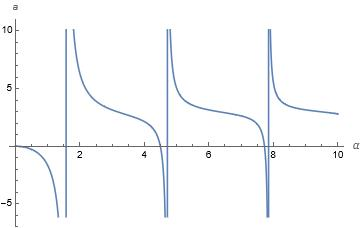
\includegraphics{3d_scattering.jpg}
\end{figure}

可以看到,势$\alpha$随散射长度$a$的变化,当$\alpha_c=(2n+1)\pi/2$时,$a$出现奇异性,对应着束缚态的出现。

\subsubsection{3D散射中的$\delta$函数}

我们首先给出3D散射下散射振幅
\begin{align}
   f=\frac{1}{k\mbox{cot}\delta-\mbox{i}k}
\end{align}
观察(\ref{3d_m}),由于$\alpha$是$\mO$(1),因此$a\sim\mO(\Delta)$,因此当势阱宽度趋于0时,散射振幅也趋于0,这种相互作用称为无关相互作用。因此无法用$\delta$函数来模拟球势阱。

如果我们用场$\psi$表示散射粒子,拉氏密度为
\begin{align}
   \mL = \psi^{\dagger}\Big(\mbox{i}\partial_t+\frac{\nabla^2}{2M}\Big)\psi-\frac{C_0}{4}\Big(\psi^{\dagger}\psi\Big)^2
\end{align}


\section{手征拉氏量}
该章主要参考\cite{scherer2011primer}

首先QCD的拉氏量具有如下形式(仅考虑u、d、s夸克)
\begin{align}
   \mL=\sum_{i=1}^{3}(\bar{q}_i \mbox{i} \slashed{D} q_i-m_i \bar{q}_i q_i)-\frac{1}{4}\mathcal{G}_{\mu \nu}^a \mathcal{G}^{a \mu \nu} 
\end{align}
其中$D_{\mu}=\partial_{\mu}-\mbox{i} g T^a A_{\mu}^a,\ T^a=\lambda^a/2$。仅考虑动能项时,具有$U(3)_L \times U(3)_R$的对称性。量子化之后$U(1)_A$被破坏,系统的对称群为$SU(3)_L \times SU(3)_R \times U(1)_V$,其中$U(1)_V$对应着重子数。由于质量项的存在,$SU(3)_L \times SU(3)_R$遭到了破坏,但当粒子质量相同时,依旧会保持$SU(3)_V$的对称性。

考虑质量项,
\begin{align}
   \sum_{i} m_i \bar{q}_i q_i = \sum_{i,j} \bar{q}_{R,i} M_{ij} q_{L,j}
\end{align}
其中$M=diag(m_u,m_d,m_s)$。如果我们将质量项升级为场,在最后结果的时候在取回常数,并假设其在手征变换下进行如下变换,
\begin{align}
   M \to RML^{\dagger}
\end{align}
则拉氏量依然在$SU(3)_L \times SU(3)_R$变换下不变。

除质量项的显式破缺外,当考虑夸克凝聚的时候,也会产生自发破缺,考虑QCD真空
\begin{align}
   \langle 0 | \bar{q}_{R,i} q_{L,j}| 0 \rangle =\Lambda ^3 \delta_{ij}
\end{align}
其中$\Lambda$具有质量量纲。其在$SU(3)_L \times SU(3)_R$下按照$(3,\bar{3})$变换。
在手征变换下,
\begin{align}
   L_{im}\langle 0 | \bar{q}_{R,n} q_{L,m}| 0 \rangle R^{\dagger}_{nj}=\Lambda ^3 U_{ij}
\end{align}
其中$U_{ij}=(LR^{\dagger})_{ij}$。当$L=R$时,真空没有变化,此时恰好对应$SU(3)_V$。

我们可以采用和质量类似的方式,将$U$升格为场,并将其参数化为
\begin{align}
   U(x)=exp[\frac{i}{f} \phi(x)],\ \phi(x)=T^a \phi^a(x)
\end{align}
其中,$\phi^a(x)$为破缺生成的8个Goldstone玻色子。

当N=2时,
\begin{align}
   \phi \equiv \sum_{i=1}^{3} \phi_a \sigma^a =
   \begin{pmatrix}
      \phi_3 & \phi_1 - \mbox{i} \phi_2 \\
      \phi_1 + \mbox{i} \phi_2) & -\phi_3
   \end{pmatrix}
   =\begin{pmatrix}
      \pi^0 & \sqrt{2}\pi^+ \\
      \sqrt{2}\pi^- & \pi^0
   \end{pmatrix}
\end{align}

当N=3时,
\begin{align}
   \phi \equiv \begin{pmatrix}
      \pi^0+\frac{\eta}{3} & \sqrt{2}\pi^+ & \sqrt{2}K^+ \\
      \sqrt{2}\pi^- & -\pi^0+\frac{\eta}{3} &\sqrt{2}K^0 \\
      \sqrt{2}K^- & \sqrt{2}\bar{K}^0 & -\frac{2\eta}{3}
   \end{pmatrix}
\end{align}

\subsection{流代数}
   在正式考虑手征拉氏量的写法之前,我们首先讨论与手征相关的流代数。
在手征极限下,拉氏量可以写为
\begin{align}
   \mL_{0} = \sum_{l=u,d,s} (\bar{q}_{R,l} \mbox{i}\slashed{D} q_{R,l} + \bar{q}_{L,l} \mbox{i}\slashed{D} q_{L,l}) -\frac{1}{4}\mathcal{G}_{a\mu\nu}\mathcal{G}_a^{\mu\nu}
\end{align}
在$U(3)_L \times U(3)_R$群下,场的变化如下
\begin{align*}
   \begin{pmatrix}
      u_L\\
      d_L\\
      s_L
   \end{pmatrix}
   \mapsto U_L
   \begin{pmatrix}
      u_L\\
      d_L\\
      s_L
   \end{pmatrix}
   =
   exp\left(-\mbox{i}\sum_{a=1}^{8}\Theta_{La}\frac{\lambda_a}{2}\right)
   e^{-\mbox{i}\Theta_L}
   \begin{pmatrix}
      u_L\\
      d_L\\
      s_L
   \end{pmatrix}
\end{align*}

\begin{align}
   \begin{pmatrix}
      u_R\\
      d_R\\
      s_R
   \end{pmatrix}
   \mapsto U_R
   \begin{pmatrix}
      u_R\\
      d_R\\
      s_R
   \end{pmatrix}
   =
   exp\left(-\mbox{i}\sum_{a=1}^{8}\Theta_{Ra}\frac{\lambda_a}{2}\right)
   e^{-\mbox{i}\Theta_R}
   \begin{pmatrix}
      u_R\\
      d_R\\
      s_R
   \end{pmatrix}
\end{align}
则拉氏量的变换为
\begin{align}
   \delta \mL_0 = \bar{q}_R \left(\sum_{a=1}^8\partial_{\mu}\varepsilon_{Ra}\frac{\lambda_a}{2}+\partial_{\mu}\varepsilon_R\right)\gamma^{\mu} q_R + \bar{q}_L \left(\sum_{a=1}^8\partial_{\mu}\varepsilon_{La}\frac{\lambda_a}{2}+\partial_{\mu}\varepsilon_R\right)\gamma^{\mu} q_L
\end{align}
因此产生的左手流和右手流分别为
\begin{align}
   \begin{aligned}
      L^{\mu}_a &= \bar{q}_L\gamma^{\mu}\frac{\lambda_a}{2}q_L, R^{\mu}_a = \bar{q}_R\gamma^{\mu}\frac{\lambda_a}{2}q_R \\
      L^{\mu} &= \bar{q}_L\gamma^{\mu}q_L, R^{\mu} = \bar{q}_R\gamma^{\mu}q_R
   \end{aligned}
\end{align} 
其中带有下指标$a$的流称为八重态,不带有的称为单态。
定义两个单态矢量流和轴矢流为
\begin{align}
   V^{\mu} = R^{\mu} + L^{\mu} = \bar{q}\gamma^{\mu}q, 
   A^{\mu} = R^{\mu} - L^{\mu} = \bar{q}\gamma^{\mu}\gamma_5  q 
\end{align}
定义两个八重态矢量流和轴矢流为
\begin{align}
   V_a^{\mu} = R_a^{\mu} + L_a^{\mu} = \bar{q}\gamma^{\mu}\frac{\lambda_a}{2} q, 
   A_a^{\mu} = R_a^{\mu} - L_a^{\mu} = \bar{q}\gamma^{\mu}\gamma_5 \frac{\lambda_a}{2} q 
\end{align}
单态矢量流即使在量子化之后依旧守恒,对应重子数守恒,而单态轴矢流在量子化之后出现反常。

定义三个荷算符
\begin{align}
   \begin{aligned}
      Q_{La}(t) &= \int \mbox{d}^3x q_L^{\dagger}(t,\vec{x}) \frac{\lambda_a}{2}q_L(t,\vec{x})\\
      Q_{Ra}(t) &= \int \mbox{d}^3x q_R^{\dagger}(t,\vec{x}) \frac{\lambda_a}{2}q_R(t,\vec{x})\\
      Q_{V}(t) &= \int \mbox{d}^3x q^{\dagger}(t,\vec{x}) q(t,\vec{x})
   \end{aligned}   
\end{align}
三个荷算符之间的对易关系恰好对应着$SU(3)_L\times SU(3)_R\times U(1)_V$的李代数
\begin{align}
   \begin{aligned}
      [Q_{La},Q_{Lb}]=\mbox{i}f_{abc}Q_{Lc}, [Q_{Ra},Q_{Rb}]=\mbox{i}f_{abc}Q_{Rc}\\
      [Q_{La},Q_{Rb}]=[Q_{La},Q_V]=[Q_{Ra},Q_V]=0
   \end{aligned}
\end{align}



\subsection{Goldstone玻色子的实现}

  























    
\newpage 

\renewcommand\refname{参考文献}

\bibliographystyle{unsrt}

\bibliography{ChPT}

\end{document}
